\subsection{Core value}
\begin{table}[!ht]
	\begin{tabular}{| l | l | l | l | l | l |}
	  \hline			
	  dataset & id = 0 & id = 17 & id = 9422 & id = 18475 & id = 27763 \\ \hline
	  soc-Slashdot0811 & 43 & 43 & 43 & 43 & 15\\ \hline
	  soc-Epinions1 & 67 & 43 & 2 & 10 & 4 \\
	  \hline  
	\end{tabular}
	\label{tab:a}
\end{table}

\subsection{Degeneracy value}
soc-Slashdot0811 : 55\\
soc-Epinions1 : 67\\


\subsection{Core value distribution}
\begin{figure}[H]
\minipage{0.48\textwidth}
  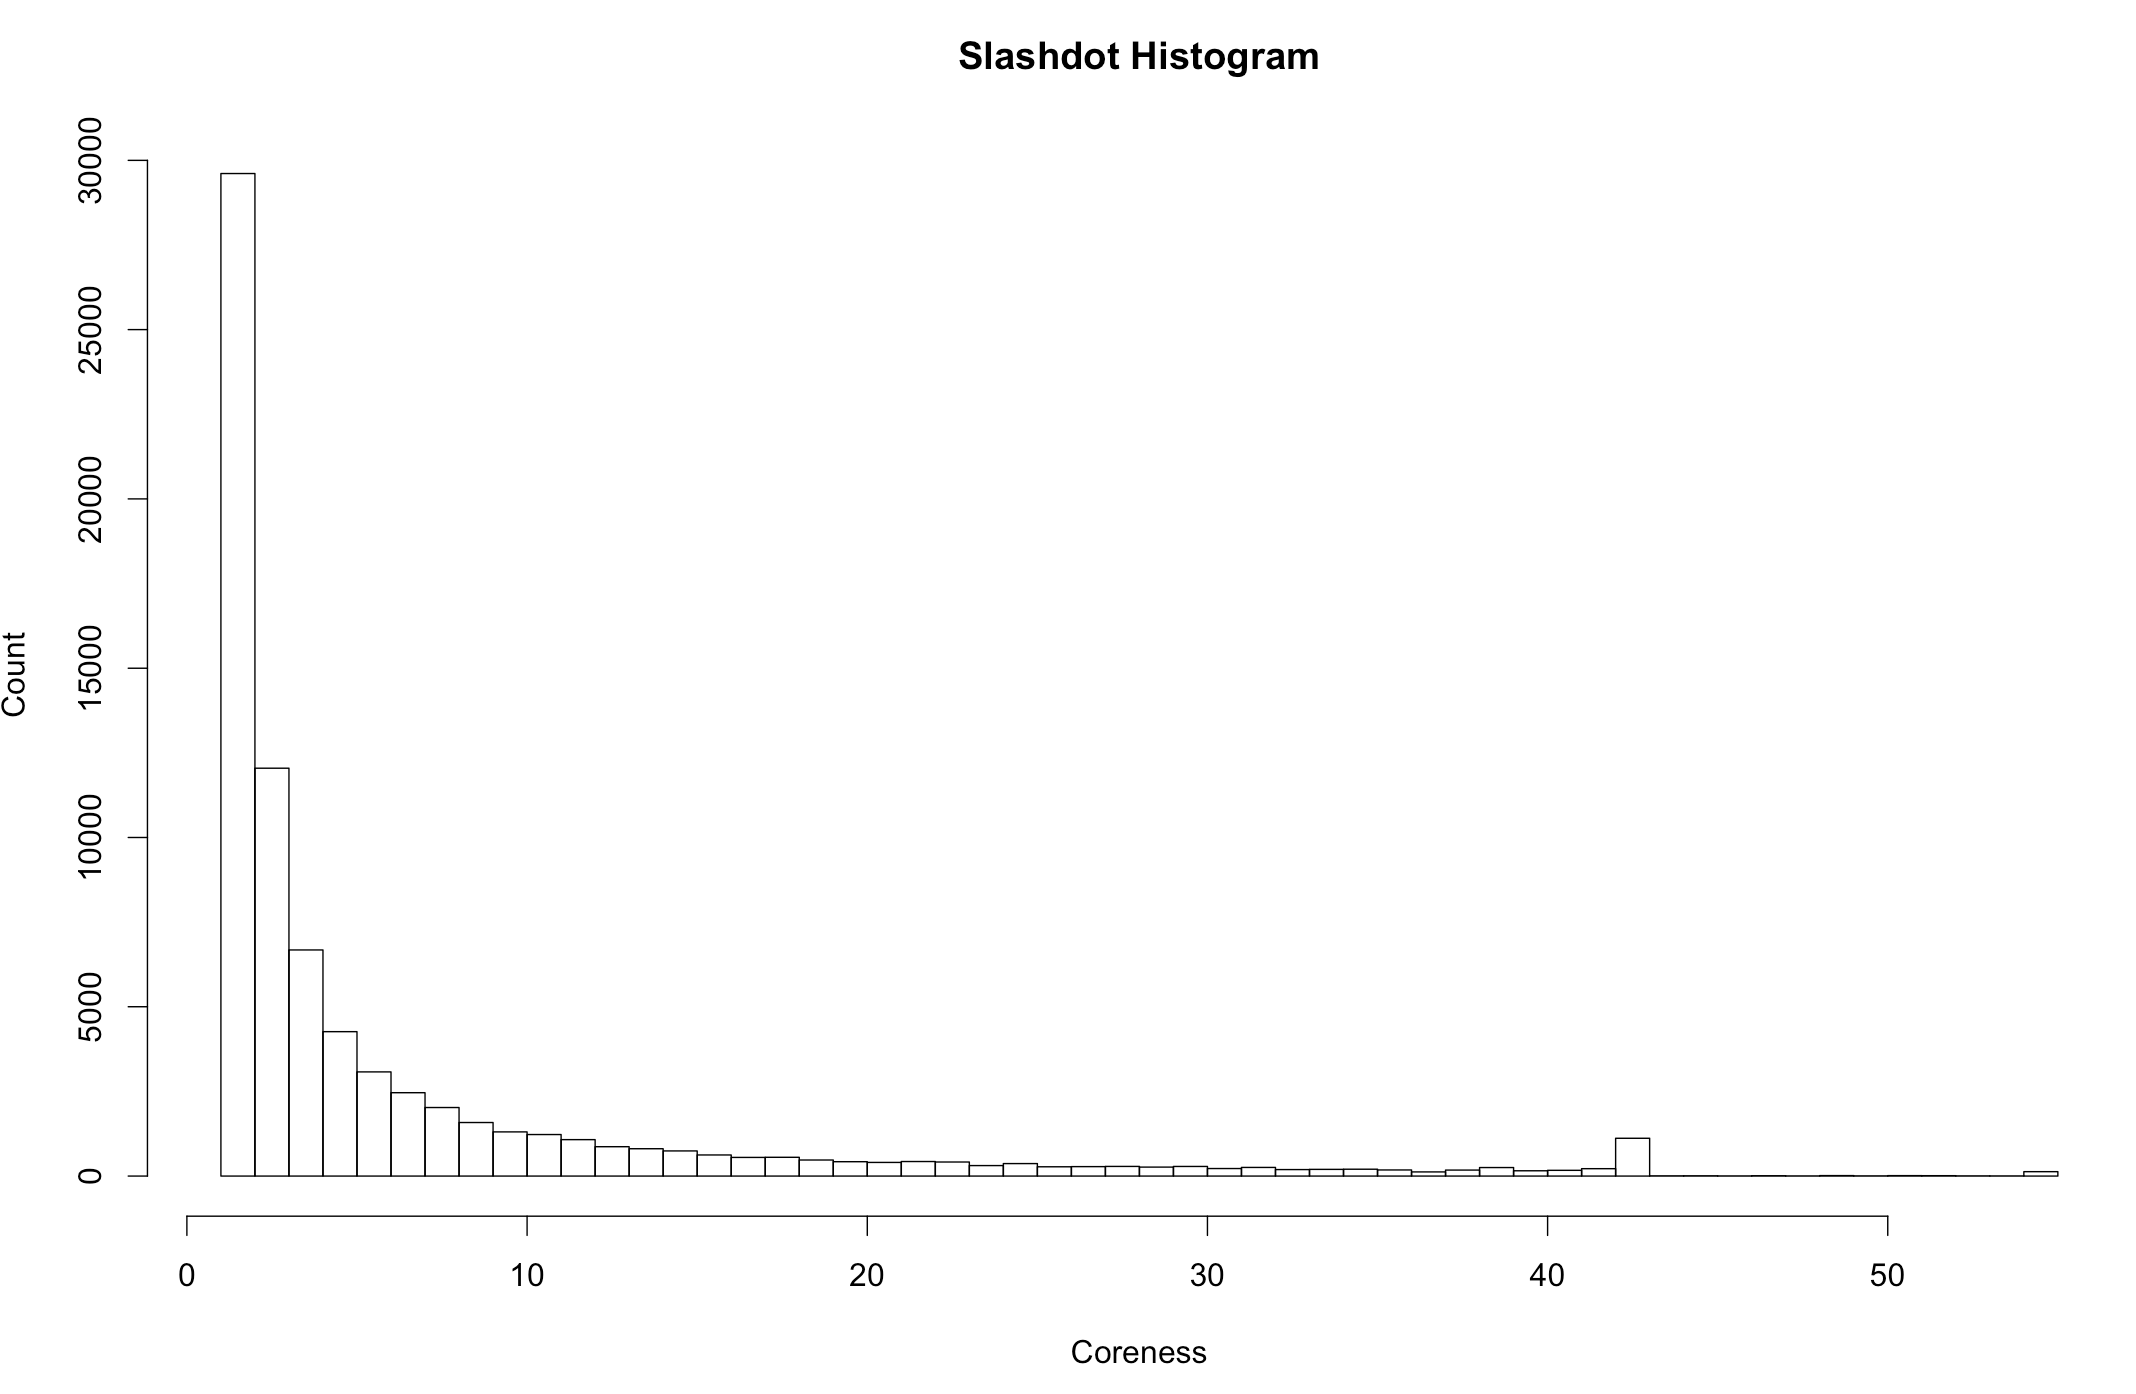
\includegraphics[width=\linewidth]{hist1}
  \caption{soc-Slashdot0811}
\endminipage\hfill
\minipage{0.48\textwidth}
  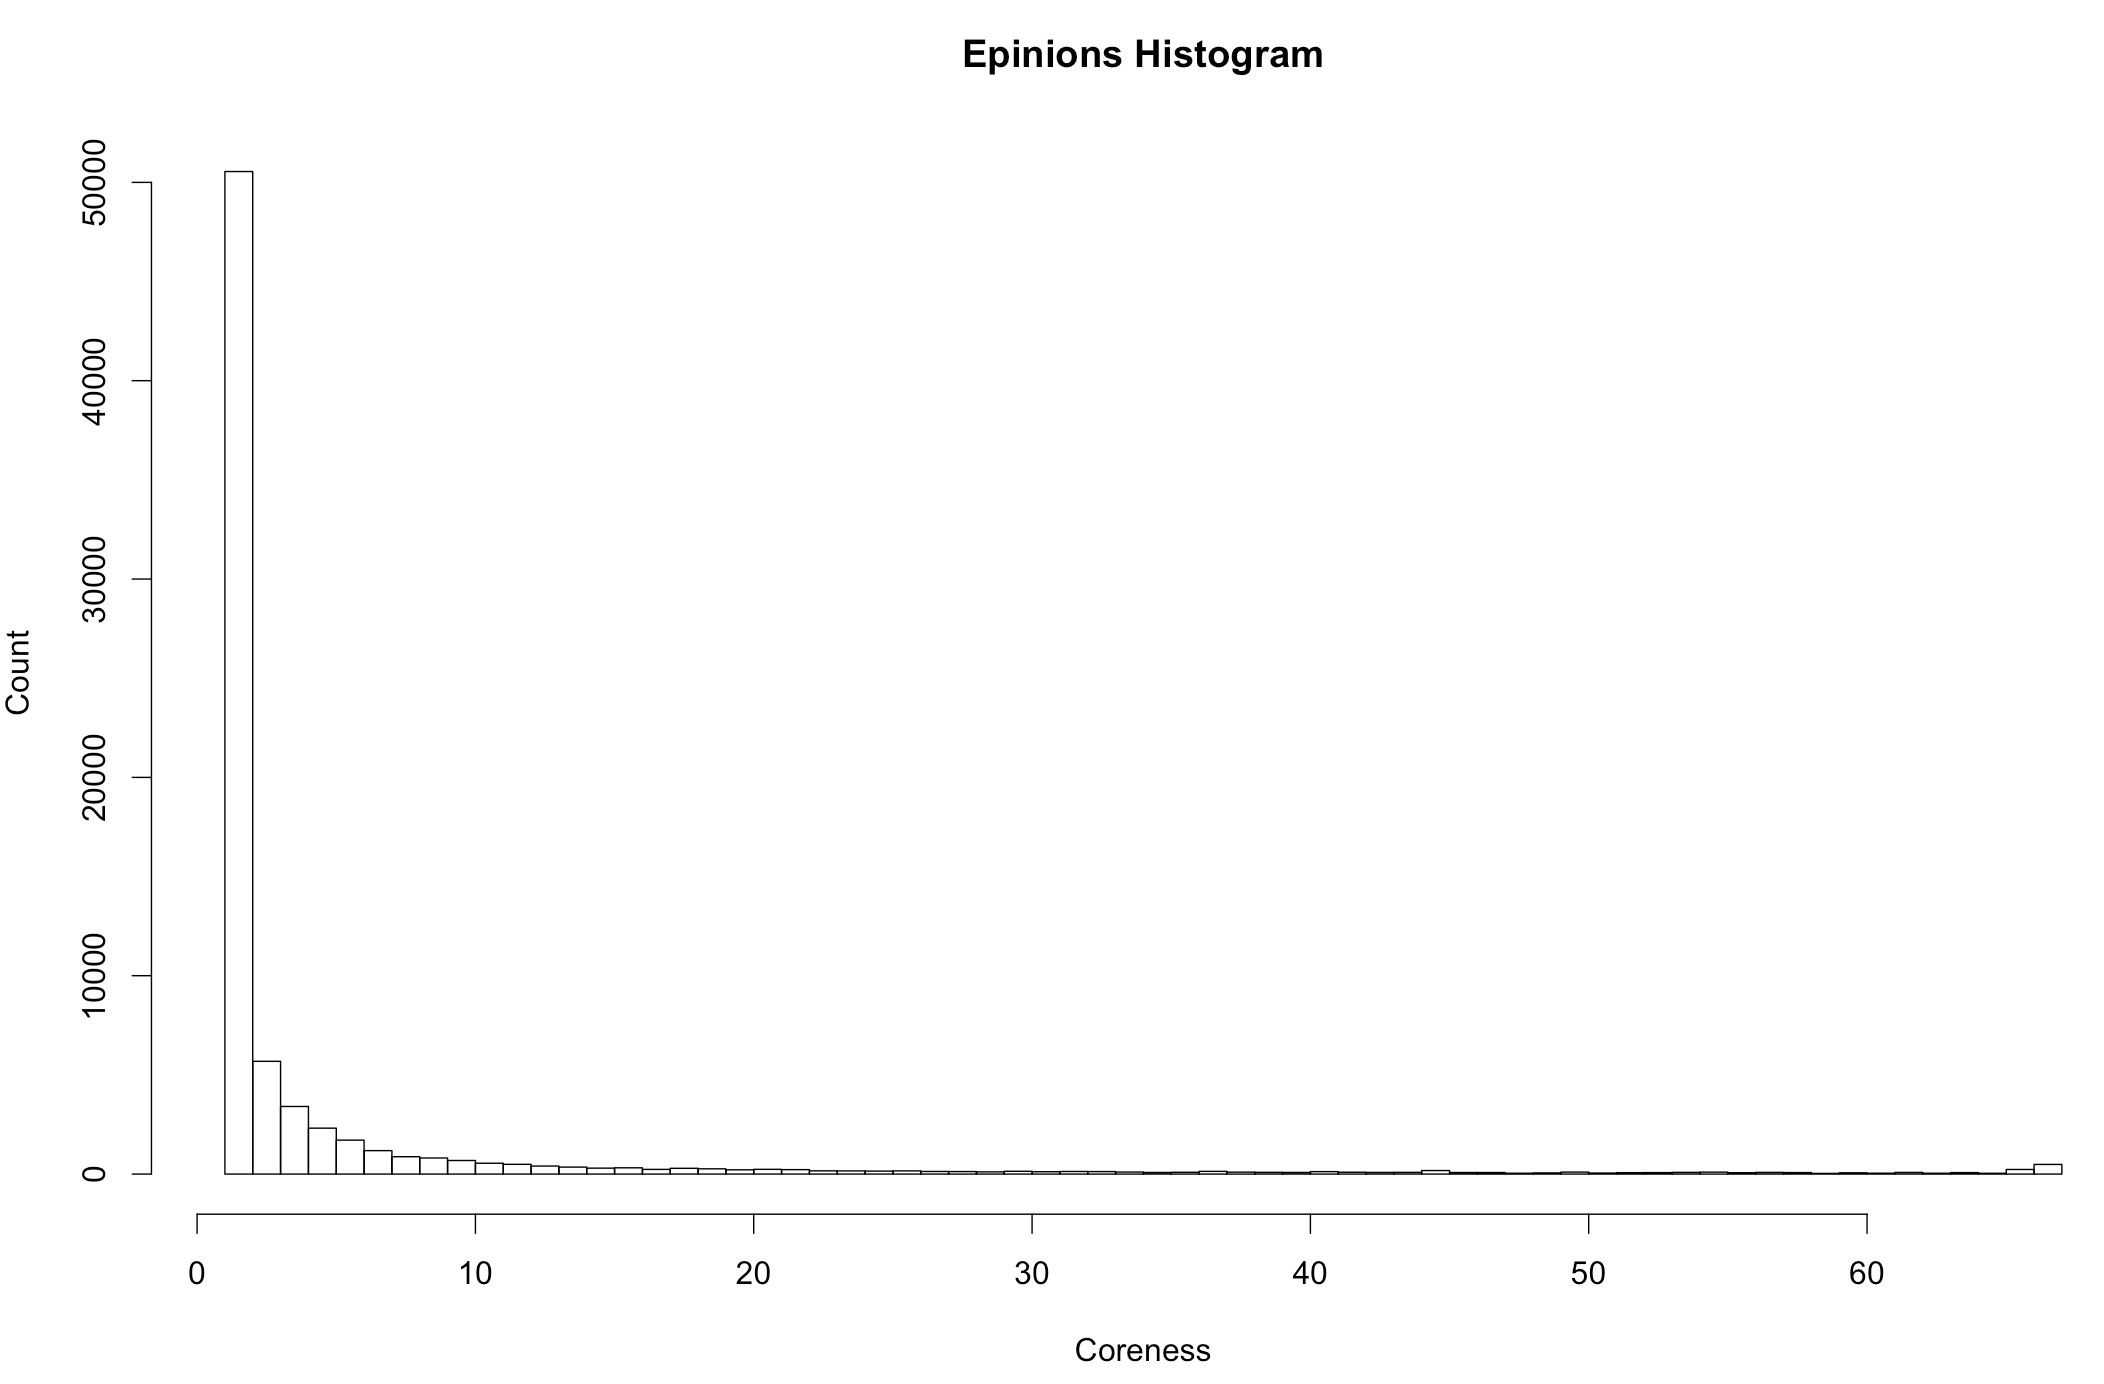
\includegraphics[width=\linewidth]{hist2}
  \caption{soc-Epinions1}
\endminipage
\end{figure}